\subsubsection{\'Equilibrage automatique NUMA}
Les noyaux Linux récents proposent un équilibrage de charge automatique des pages mémoires.
%
Malheureusement, nous ne pouvons pas utiliser les grappes de serveurs à notre disposition pour tester cette fonctionnalité.
%
La version de Linux disponible sur ces machines n'est pas assez récente, la fonctionnalité AutoNUMA n'est apparue que dans la version 3.13 du noyau.
%
\`A la place, nous allons utiliser une machine de bureau contenant deux processeurs Intel Xeon X5660, chaque banc NUMA dispose de 6 coeurs de calculs et de 24~Go de mémoire vive.
%
La version de Linux utilisée est la 3.18.

Cette méthode ne fonctionne que lorsque le programme est exécuté suffisamment longtemps pour avoir le temps d'analyser toute la mémoire utilisée.
%
Nous allons chercher l'accélération maximale que nous pouvons atteindre avec cette solution.
%
Il ne nous est donc pas utile de faire varier le nombre de coeurs de calcul, nous utiliserons les 12 coeurs de calcul de la machine.
%
Nous allons plutôt faire varier le nombre de SpMV pour faire varier le temps d'exécution du programme et laisser au noyau assez de temps pour déplacer les pages.

%   (-_-)   %
\begin{figure}
  \centering
  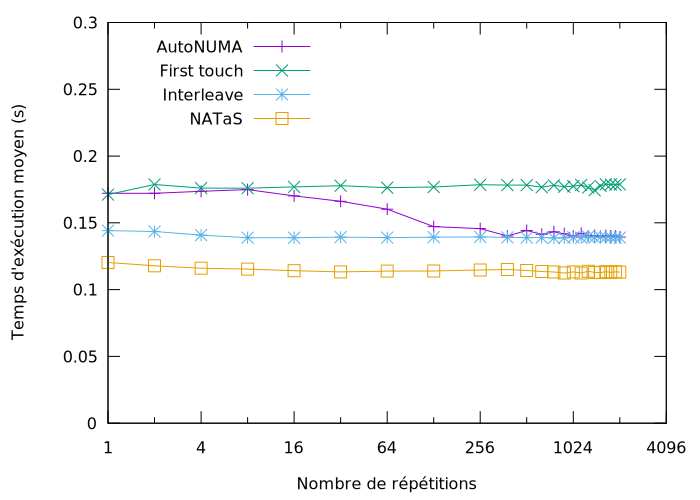
\includegraphics[width=0.7\textwidth]{res_spmv_frep}
  \caption{Temps d'un produit matrice vecteur creux sur Linux 3.18 en mémoire partagée avec 12 coeurs. Nous utilisons une matrice représentant un cube 100 avec 8 variables primaires.}
  \label{fig:res_spmv_frep}
\end{figure}

Avec un nombre de répétitions faibles, AutoNUMA donne les mêmes performances que l'allocation first touch (Fig.~\ref{fig:res_spmv_frep}).
%
Au bout de 8 répétitions, soit environ 1,36~seconde, nous commençons à voir une amélioration des performances.
%
Vers 384 répétitions, soit environ 1 minute, nous obtenons la performance crête d'AutoNUMA qui correspond aussi à la performance obtenue avec l'allocation interleave.
%
Il est nécessaire de rappeler que l'allocation interleave donnait de bonnes performances avec l'utilisation de 2 bancs NUMA.
%
Les meilleurs résultats sont obtenus avec NATaS.
%
Il serait aussi intéressant de tester la méthode AutoNUMA sur Manumanu en utilisant plus de 2 bancs NUMA, nous pourrions savoir si les résultats sont meilleurs qu'avec NATaS.
%
Malheureusement, nous ne pouvons pas changer le noyau utilisé sur cette machine.
